% EJB

\begin{frame}{Exemple de modèle de programmation: EJB}
  \begin{center}
    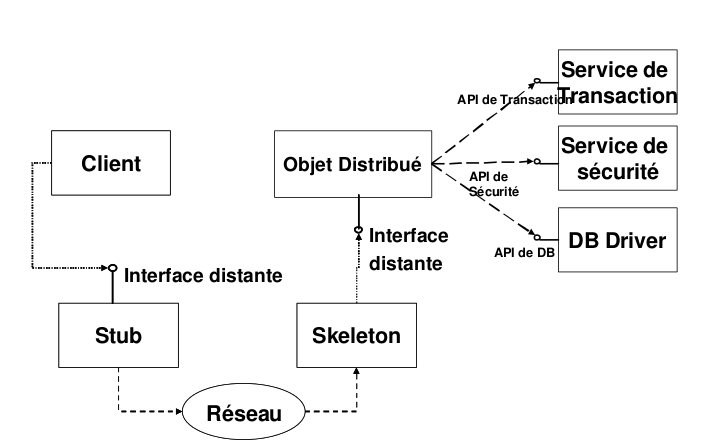
\includegraphics[scale=0.3]{img/ejb-overview.png}
  \end{center}
\end{frame}


\begin{frame}
  \begin{block}{Motivations}
    \begin{itemize}
      \item EJB définit des contrats associés à un Bean
      \item Déploiement local ou distant
    \end{itemize}
  \end{block}

  \begin{block}{Standard}
     \begin{itemize}
       \item Portabilité des beans sur différents serveurs EJB
       \item Indépendance du fournisseur
    \end{itemize}
  \end{block}
\end{frame}

\begin{frame}
  \begin{block}{Types}
    \begin{itemize}
      \item Session Bean
      \item Entity Bean
      \item Message-Driven Bean
    \end{itemize}
  \end{block}

  \begin{center}
    Si l'on utilise un Session Bean quel impact sur l'architecture de l'application ?
  \end{center}

\end{frame}
